\chapter{数据结构基础}
\section{线性数据结构}
\subsection{数组}
\subsection{链表}
\subsection{栈}
\subsection{队列}
\section{非线性数据结构}
\subsection{树}
\subsubsection{二叉树的遍历}
\paragraph{先序遍历}
\begin{lstlisting}{language=c++}
	void  PreOrderTraversal(BTree *tree) {
	if (bt == NULL)  {
		return ; 
	}
	VISIT(bt);
	PreOrderTraversal(tree->left); 
	PreOrderTraversal(tree->right); 
}

\end{lstlisting}
\paragraph{中序遍历}
\begin{lstlisting}{language=c++}
	void InorderTraversal(BTree *tree) {
		if (bt == NULL)  {
			return ; 
		}
		InorderTraversal(tree->left); 
		VISIT(bt);
		InorderTraversal(tree->right); 
	}
\end{lstlisting}

\paragraph{后序遍历}
\begin{lstlisting}{language=c++}
	void PostOrderTraversal(BTree *tree) {
		if (bt == NULL)  {
			return ; 
		}
		PostOrderTraversal(tree->left); 
		PostOrderTraversal(tree->right); 
		VISIT(bt);
	}
\end{lstlisting}
\subsubsection{二叉树的增删改查}

\subsection{跳跃表}
\subsection{图}
\subsection{散列表}
\paragraph{LRUCcache的实现} 
设计并实现一个满足  LRU (最近最少使用) 缓存 约束的数据结构。
\paragraph{实现 LRUCache 类:}
\begin{itemize}
\item  LRUCache(int capacity) 以 正整数 作为容量 capacity 初始化 LRU 缓存
\item int get(int key) 如果关键字 key 存在于缓存中,则返回关键字的值,否则返回 -1 。
\item void put(int key, int value) 如果关键字 key 已经存在,则变更其数据值 value ;如果不存在,则向缓存中插入该组 key-value 。
\item 如果插入操作导致关键字数量超过 capacity ,则应该 逐出 最久未使用的关键字。
\item 函数 get 和 put 必须以 O(1) 的平均时间复杂度运行。
\end{itemize}
\begin{lstlisting}
type DLinkedNode struct {
	Prev *DLinkedNode
	Next *DLinkedNode
	Key  int
	Val  int
}

type LRUCache struct {
	head, tail *DLinkedNode
	size       int
	capacity   int // 队列最大长度
	cache      map[int]*DLinkedNode
}

func Constructor(capacity int) LRUCache {
	l := LRUCache{
		head:     initDLinkedNode(0, 0),
		tail:     initDLinkedNode(0, 0),
		capacity: capacity,
		cache:    make(map[int]*DLinkedNode),
	}
	
	l.head.Next = l.tail
	l.tail.Prev = l.head
	return l
}

func initDLinkedNode(key, val int) *DLinkedNode {
	return &DLinkedNode{
		Key: key,
		Val: val,
	}
}

func (this *LRUCache) moveToHead(node *DLinkedNode) {
	this.removeNode(node)
	this.addToHead(node)
	return
}

func (this *LRUCache) removeNode(node *DLinkedNode) {
	prev := node.Prev
	next := node.Next
	prev.Next = next
	next.Prev = prev
	return
}

// 链表都是带虚拟头节点的
func (this *LRUCache) addToHead(node *DLinkedNode) {
	node.Prev = this.head
	node.Next = this.head.Next
	this.head.Next.Prev = node
	this.head.Next = node
	return
}

func (this *LRUCache) removeTail() *DLinkedNode {
	node := this.tail.Prev
	this.removeNode(node)
	return node
}

func (this *LRUCache) Get(key int) int {
	if _, ok := this.cache[key]; !ok {
		return -1
	}
	
	node := this.cache[key]
	this.moveToHead(node)
	return node.Val
}

func (this *LRUCache) Put(key int, value int) {
	if node, ok := this.cache[key]; ok {
		node.Val = value
		this.moveToHead(node)
		return
	}
	
	if this.size >= this.capacity {
		removed := this.removeTail()
		delete(this.cache, removed.Key)
		this.size--
	}
	node := &DLinkedNode{Key: key, Val: value}
	this.addToHead(node)
	this.cache[key] = node
	this.size++
	return
}

\end{lstlisting}
\subsection{邻接矩阵}

\section{查找}
\subsection{二分查找}
\section{排序}
\subsection{快速排序}
\paragraph{算法一书对快排的解释} 
\paragraph{快速排序的发明人}Robert Sedgewick , 《算法》一书的作者, 同时也是红黑树的发明人, 同时解决了shell排序、堆排序。 曾经做过Donald Knuth 的顾问, 并在高德纳那里拿到了博士学位, 他的博士学位论文就是quicksort 关于Rober Sedgewick 的wiki网页 
\href{https://en.wikipedia.org/wiki/Robert_Sedgewick_(computer_scientist)} {RoberSedgewick}

\paragraph{关键思想}快速排序的关键是划分算法, 从《计算机程序设计艺术》 引用了R.Sedgewick的划分方法。 

\newpage
\begin{lstlisting}{language=c++}

func quicksort(a []int) {
	l, r := 0, len(a)-1
	qsort(a, l, r)
	return
}
func qsort(a []int, l, r int) {
	if l >= r {
		return
	}
	q := partition(a, l, r)
	fmt.Printf("l=%d, q=%d, r=%d \n", l, q, r)
	qsort(a, l, q)
	qsort(a, q+1, r)
	
}
\end{lstlisting}
\newpage
\paragraph{Robert Sedgewick 在算法一书提到的划分方法}
一般策略是先 随意地取a[lo]作为切分元素,即那个将会被排定的元素, 然后我们从数组的左端开始向右扫描直到找到一个大于等 于它的元素,再从数组的右端开始向左扫描直到找到一个 小于等于它的元素。这两个元素显然是没有排定的,因此 我们交换它们的位置。如此继续,我们就可以保证左指针 i 的左侧元素都不大于切分元素,右指针 j 的右侧元素都 不小于切分元素。当两个指针相遇时,我们只需要将切分 元素 a[lo] 和左子数组最右侧的元素(a[j])交换然后返 回 j 即可。切分方法的大致过程如图\ref{Fig.algo_qsort} 所示。

\newpage
\begin{figure}
\label{Fig.algo_qsort}
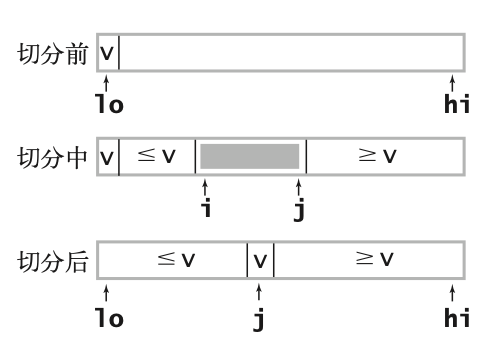
\includegraphics[width=0.9\textwidth]{./images/quicksort_partiton_algo4.png}
\caption{algo4一书的描述的划分方法}
\end{figure}
\begin{lstlisting}
func partition(arr []int, p, r int) int {
	pivot := arr[p]
	i, j := p+1, r
	for {
		for arr[i] < pivot {
			i++
			if i == r {
				break
			}
		}
		
		for pivot < arr[j] {
			j--
			if j == p {
				break
			}
		}
		if i >= j {
			break
		}
		exch(arr, i, j)
	}
	//	fmt.Printf("[p=%d] j=%d arr= %+v\n", pivot, j, arr)
	exch(arr, p, j)
	return j
}

func exch(a []int, i, j int) {
	a[i], a[j] = a[j], a[i]
}

\end{lstlisting}

\paragraph{基于Lomuto快排划分算法}
基本思想: j指针左侧是小于pivot的数, 右侧是大于pivo的数 , i向前探索,如果遇到小于pivot, j指针向前,表示j的边界扩展,  交换i,j位置的数 ,直到全部处理完成。 最后将pivot位置的数和j位置的数交换


\begin{figure}
	\centering
	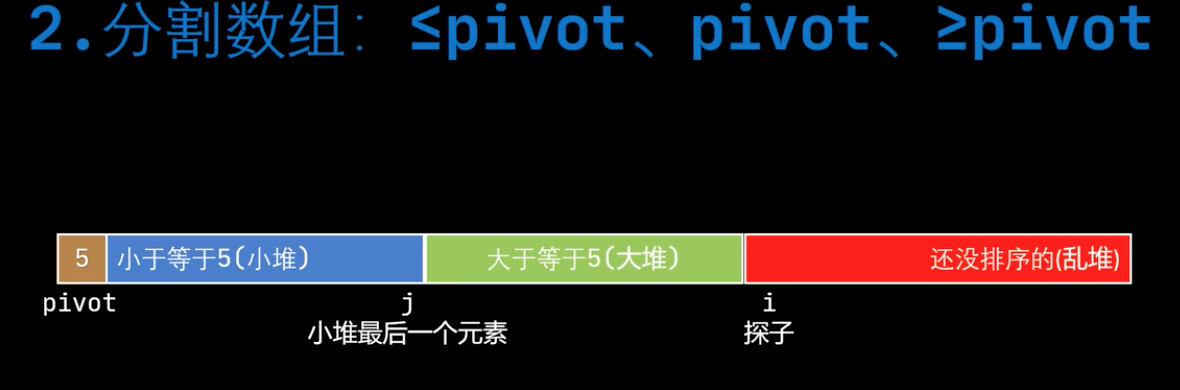
\includegraphics[width=0.9\textwidth]{./images/lomuto_qsort_think.png}
	\caption{基于Lomuto快排划分算法}
\end{figure}
\begin{lstlisting}
func partition(a []int, l, r int) int {
	
	pivot := a[l]
	j := l
	for i := l; i <= r; i++ {
		if a[i] < pivot {
			j++
			a[i], a[j] = a[j], a[i]
		}
	}
	
	a[l], a[j] = a[j], a[l]
	return j
}
\end{lstlisting}


\begin{lstlisting}
	内容...
\end{lstlisting}

\subsection{归并排序}
\subsection{插入排序}
\subsection{希尔排序}
\subsection{基数排序}
\subsection{桶排序}

